\documentclass[a4paper]{article}

\usepackage[utf8]{inputenc}
\usepackage[portuguese]{babel}
\usepackage{a4wide}
\usepackage[pdftex]{hyperref}
\usepackage{graphicx}
\usepackage{wrapfig}
\usepackage{amsmath}
\usepackage{verbatim}
\usepackage{caption}
\usepackage{subcaption}
\usepackage{float}



\begin{document}

\begin{titlepage}
\begin{center}



\includegraphics[width=0.6\textwidth]{logo.jpg}\\[0.5cm]

{\large Universidade do Minho - Escola de Engenharia}\\[0.5cm]

{\large Relatório do trabalho prático de Sistemas Distribuídos}\\[0.5cm]

% Title
\rule{\linewidth}{0.5mm} \\[0.4cm]
{ \huge \bfseries Matchmaking num jogo online \\[0.4cm] }
\rule{\linewidth}{0.5mm} \\[1.5cm]

% Author and supervisor
\noindent
\begin{minipage}{0.4\textwidth}
  \begin{flushleft} \large
    \emph{Autores :}\\
    Daniel Maia \textsc{(A77531)}\\
    
\includegraphics[width=1.5cm]{daniel.jpg}\break
    Diogo Silva\textsc{(A78034)}\\
    
\includegraphics[width=1.5cm]{afonso.jpg}\break
    Marco Silva\textsc{(A79607)}\\
    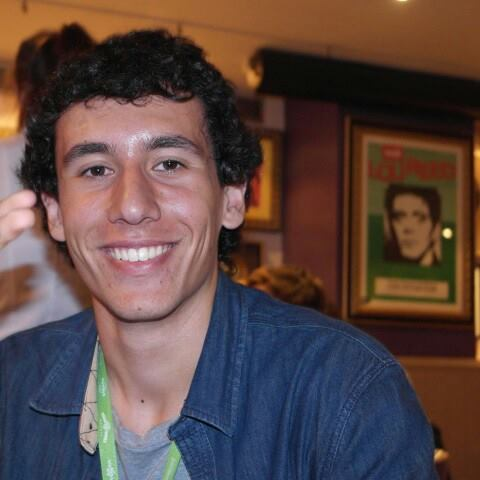
\includegraphics[width=1.5cm]{marco.jpg}\break
  \end{flushleft}
\end{minipage}%
\vfill

% Bottom of the page
{\large Versão 1.0 \\ \today}

\end{center}
\end{titlepage}




\begin{abstract}

\hspace{3mm} 

\end{abstract}

\pagebreak
\tableofcontents

\pagebreak
\section{Introdução}
\label{sec:1}

\hspace{3mm} 



%------------------------------------------------------------------------

\pagebreak
\section{Descrição do problema}
\label{sec:2}

\hspace{3mm} A proposta de trabalho dada para o projeto é o da implementação de uma aplicação distribuída para \textit{matchmaking} num jogo \textit{online}, num estilo semelhante a videojogos tais como Overwatch ou Paladins. Esta aplicação terá a capacidade de, nomeadamente, formar automaticamente duas equipas por partida e permitir a cada jogador um intervalo de tempo para escolher uma personagem, referida como herói, antes da partida iniciar.

\par Cada equipa será constituída por 5 jogadores, cada um com uma classificação pessoal. Esta classificação, determinada pelas vitórias e derrotas sofridas no jogo, terá um valor inteiro entre 0 e 9, e será semelhante em valor entre todos os jogadores de uma dada partida. 


\pagebreak
\clearpage
%--------------------------------------------------------------------------

\section{Conceção da Solução}
\label{sec:3}

\subsection{Registo e login}

\hspace{3mm} 



\subsection{Matchmaking}

\hspace{3mm} 




\subsection{Fazer equipas}

\hspace{3mm} 

\subsection{Escolha de heróis}

\hspace{3mm} 

\subsection{Cálculo dos resultados}

\hspace{3mm} 

\pagebreak

%--------------------------------------------------------------------------

\section{Conclusões}
\label{sec:4}

\hspace{3mm} 



\end{document}
